\documentclass[a4paper]{article}
\usepackage[utf8x]{inputenc}
\usepackage[T1,T2A]{fontenc}
\usepackage[russian]{babel}
\usepackage{hyperref}
\usepackage{indentfirst}
\usepackage{listings}
\usepackage{color}
\usepackage{here}
\usepackage{array}
\usepackage{multirow}
\usepackage{graphicx}
\usepackage{subcaption}

\usepackage{caption}
\renewcommand{\lstlistingname}{Программа} % заголовок листингов кода

\usepackage{listings}
\lstset{ %
extendedchars=\true,
keepspaces=true,
language=bash,					% choose the language of the code
basicstyle=\footnotesize,		% the size of the fonts that are used for the code
numbers=left,					% where to put the line-numbers
numberstyle=\footnotesize,		% the size of the fonts that are used for the line-numbers
stepnumber=1,					% the step between two line-numbers. If it is 1 each line will be numbered
numbersep=5pt,					% how far the line-numbers are from the code
backgroundcolor=\color{white},	% choose the background color. You must add \usepackage{color}
showspaces=false				% show spaces adding particular underscores
showstringspaces=false,			% underline spaces within strings
showtabs=false,					% show tabs within strings adding particular underscores
frame=single,           		% adds a frame around the code
tabsize=2,						% sets default tabsize to 2 spaces
captionpos=b,					% sets the caption-position to bottom
breaklines=true,				% sets automatic line breaking
breakatwhitespace=false,		% sets if automatic breaks should only happen at whitespace
escapeinside={\%*}{*)},			% if you want to add a comment within your code
postbreak=\raisebox{0ex}[0ex][0ex]{\ensuremath{\color{red}\hookrightarrow\space}}
}

\usepackage[left=2cm,right=2cm,
top=2cm,bottom=2cm,bindingoffset=0cm]{geometry}


\begin{document}	% начало документа

\begin{titlepage}	% начало титульной страницы

	\begin{center}		% выравнивание по центру

		\large Санкт-Петербургский Политехнический Университет Петра Великого\\
		\large Институт компьютерных наук и технологий \\
		\large Кафедра компьютерных систем и программных технологий\\[6cm]
		% название института, затем отступ 6см
		
		\huge Программирование\\[0.5cm] % название работы, затем отступ 0,5см
		\large Отчет по выполнению проекта\\[0.1cm]
		\large Космический симулятор "InSpace"\\[5cm]

	\end{center}


	\begin{flushright} % выравнивание по правому краю
		\begin{minipage}{0.25\textwidth} % врезка в половину ширины текста
			\begin{flushleft} % выровнять её содержимое по левому краю

				\large\textbf{Работу выполнил:}\\
				\large Леженин Ю.И.\\
				\large {Группа:} 23501/4\\
				
				\large \textbf{Преподаватель:}\\
				\large Вылегжанина К.Д.

			\end{flushleft}
		\end{minipage}
	\end{flushright}
	
	\vfill % заполнить всё доступное ниже пространство

	\begin{center}
	\large Санкт-Петербург\\
	\large \the\year % вывести дату
	\end{center} % закончить выравнивание по центру

\thispagestyle{empty} % не нумеровать страницу
\end{titlepage} % конец титульной страницы

\vfill % заполнить всё доступное ниже пространство



% Содержание
\tableofcontents
\newpage



\section{Космический симулятор InSpace}
\label{descr}
В современном мире существует множество различных игр-симуляторов. Один из их видов - это игры, включающие элементы экономического симулятора и предоставляющие игрокам возможность управлять экономическими системами различной степени сложности, например, городом (SimCity, Dwarf Fortress(один из режимов игры, частично), островным государством (Tropico), фермой (SimFarm), транспортной фирмой (Railroad Tycoon, OpenTTD). Данные игры, как правило, обладают сложной моделью и логикой, что обеспечивает интересный игровой процесс. Симуляторы могут предназначаться для разных платформ. Так сейчас пользуется популярностью игры данного жанра обладающие веб-интерфейсом (Ogame). Таким образом, было принято решение создать позволяющий управлять планетой космический симулятор, в который включены основные присущие этому типу игр особенности. 

\subsection{Описание игровой модели космического симулятора InSpace}

При старте игроку дается во владение планета. На планете можно возводить и улучшать здания, производить исследования и строить флот. Все перечисленные действия требуют ресурсы, добываемые на планете, некоторые здания потребляют энергию, некоторые ее производят. Исследования и здания влияют на игровой процесс, воздействуя на различные характеристики друг друга. С помощью флотов можно атаковать другие планеты и перевозить ресурсы. Подобные возможности позволяют имитировать экономическую систему. Подробное описание модели представлено ниже.

\subsubsection{Галактика и система}
Игровая модель представлена галактикой, в которой расположены непосредственно планеты. Галактика состоит из 10 систем, в каждой системе может находиться до 10 планет включительно.	

\subsubsection{Планета}
Планета дается игроку в начале игры. Она занимает какую либо позицию в системе (от 1 до 10) и имеет ограниченный размер, который исчисляется в полях для застройки. При каждом улучшении здания, количество свободных полей уменьшается. 

\subsubsection{Ресурсы}
На планете может вестись добыча трех типов ресурсов: металла, кристаллов и дейтерия. На скорость добычи ресурсов влияют уровни зданий, называемых шахтами. Для каждого типа ресурса существует своя шахта. Так же на скорость добычи может влиять уровень каких-либо исследований.

\subsubsection{Энергия и мощность}
Одни здания могут потреблять энергию, например, шахты, другие - могут ее производить. Если уровень потребляемой энергии превосходит уровень производимой, то происходит перерасчет мощности, в этом случае эффективность работы зданий уменьшается пропорционально мощности.  

\subsubsection{Здания}
В ходе игры можно улучшать здания, которые находятся на планете. В начале игры уровень каждого здания равен 0, для повышения уровня нужны ресурсы и это занимает определенный промежуток времени. С каждом уровнем количество ресурсов и времени, требуемое для улучшения, увеличивается. Количество полей, занимаемых зданием на планете, соответствует его уровню. Здания имеют различные эффекты: так, шахты влияют на добычу ресурсов, электростанция на уровень производимой энергии, лаборатория оказывает влияние на скорость проведения исследований и т.п.

\subsubsection{Исследования}
Аналогично зданиям, исследования имеют определенный уровень который можно повышать. В этом случае улучшение так же требует растущее с уровнем исследования количество ресурсов и времени. Уровень исследования не ограничен. Исследования могут обладать различным влиянием, например энергетическая технология воздействует на уровень добываемой электроэнергии. Кроме того, технологии могут воздействовать на характеристики кораблей. 

\subsubsection{Флот и корабли}
На планете можно строить корабли, которые формируют флот. Часть флота можно отправлять на миссии, также флот участвует в обороне планеты при нападении на нее вражеских кораблей. Каждый корабль обладает набором характеристик: атака, прочность, прочность щитов, скорость и вместимость ресурсов. Первые три параметра определяют боевые качества корабля. Скорость влияет на то, сколько времени потребуется кораблю на достижение какой-либо планеты. Скорость флота определяется как минимальная скорость корабля. Вместимость же показывает сколько ресурсов может перевозить корабль.

\subsubsection{Миссии}
Взаимодействие с другими планетами представлено в виде миссий. Существует разные виды миссий, например атака и транспортировка. В ходе миссии флот может атаковать другую планету и похитить часть ресурсов с нее, либо перевезти ресурсы.

%TODO

\subsection{Выводы}
Так, на основе обзора существующих симуляторов было создана небольшая игра, которая содержит элементы экономического симулятора такие, как добыча ресурсов и возможность распоряжения ими различными способами, и может быть интересна игрокам, предпочитающим данный жанр.
%Кроме того, описанная выше игровая модель содержит множество объектов, взаимодействующих друг с другом, что позволяет в ходе ее реализации использовать различные приемы проектирования и особенности используемого языка.   


\section{Проектирование приложения, реализующего космический симулятор InSpace}

\subsection{Концепция приложения} 

В качестве конечно продукта, было решено создать графическое приложение, которое должно обеспечивать игру для одного игрока. Приложение должно реализовывать все аспекты игровой механики перечисленные в разделе \ref{descr} и предоставлять возможности для удобного контроля состояния игровой модели. 

Графическое приложение состоит из окна, содержащего панель и набор кнопок для изменения содержимого этой панели. Существует несколько различных возможных вариантов содержимого панели: общая информация о планете и текущих действиях, список построек, список исследования, список кораблей, список планет в галактике. Каждый элемент графического интерфейса, должен не только предоставлять информацию о состоянии модели, но и при необходимости предоставлять возможность воздействия на нее.

\begin{figure}[H]
\centering
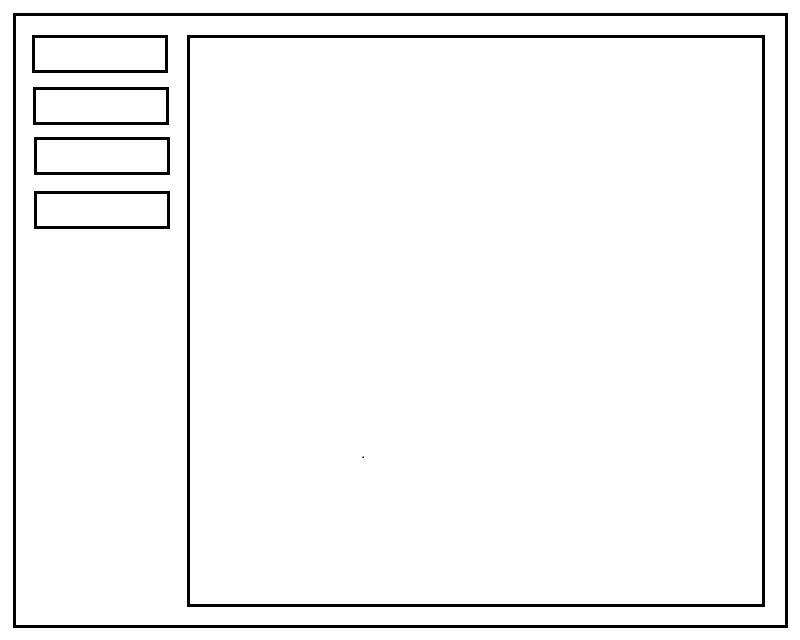
\includegraphics[scale=0.5]{sc.jpg}
\caption{Схема расположения элементов графического интерфейса}
\label{sc}
\end{figure}

На рис. \ref{sc} представлено предположительное расположение элементов графического интерфейса.

\subsection{Минимально работоспособный продукт}
Минимальным работоспособным продуктом считается реализующее игровую логику графическое приложение, рассчитанное на одного игрока.

\subsection{Прецеденты использования приложения}

В ходе работы была составлена UML диаграмма прецедентов использования.

\begin{figure}[H]
	\begin{center}
		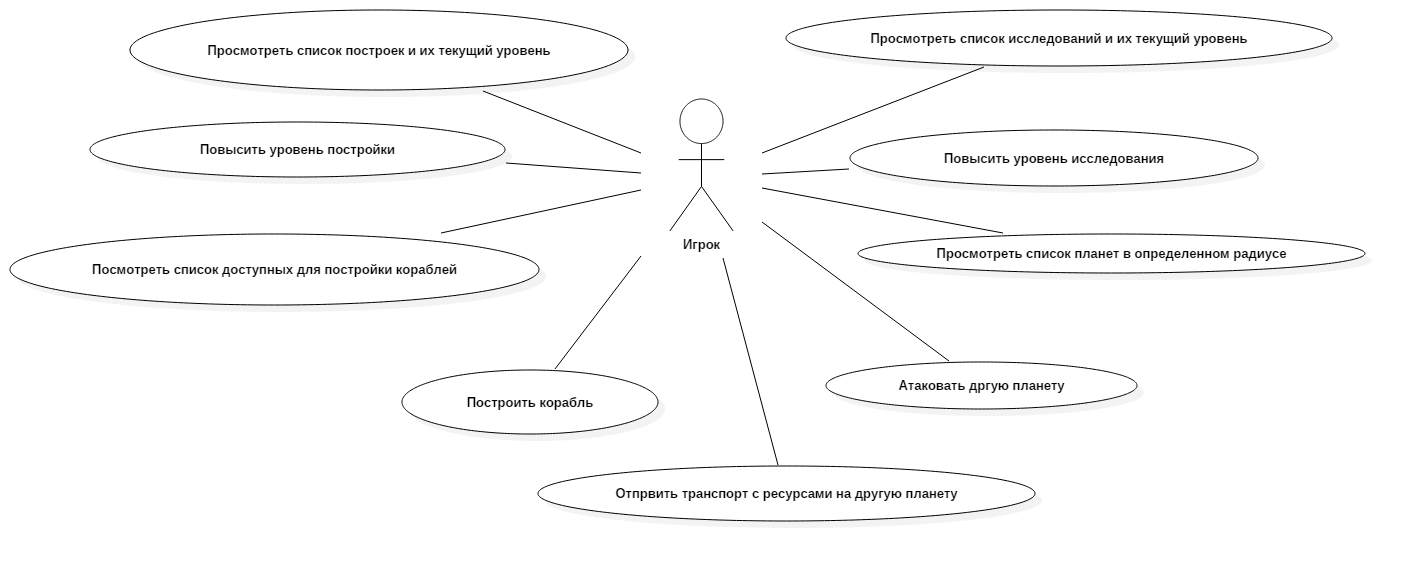
\includegraphics[scale=0.35]{../../uml/UseCaseDiagram1.png}
		\caption{Диаграмма прецедентов использования}
		\label{pic:use_case}
	\end{center}
\end{figure}

На рис. \ref{pic:use_case} перечислены основные действия совершаемые игроком, которые должны поддерживаться приложением.

\subsection{Основные компоненты приложения}

Было принято решение разделить приложение на два компонента:

\begin{enumerate}
	\item Библиотека, реализующая игровую логику
		
	 Включает в себя игровую модель и реализует игровые механизмы. В ядре должно быть обеспечено регулярное обновление модели в ответ на действие пользователя. Кроме того, должна быть реализована обработка исключительных ситуаций, включающие в себя ошибки игрока, попытки выполнить запрещенные действия и прочее. 	 
	
	\item Графическое приложение 

	Визуализирует игровую модель, предоставляет пользователю графический интерфейс для взаимодействия с ней и выполнения действий предусмотренных игровой логикой.
\end{enumerate}

\begin{figure}[H]
	\begin{center}
		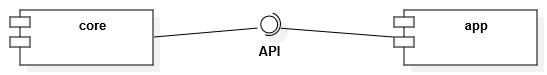
\includegraphics[scale=0.7]{../../uml/ComponentDiagram1.png}
		\caption{Диаграмма компонентов}
		\label{pic:components}
	\end{center}
\end{figure}

Так, на рис. \ref{pic:components} изображена UML диаграмма компонентов, описывающих взаимодействие компонентов. Библиотека предоставляет набор объектов, с помощью которых реализовано взаимодействие с моделью игры, так главным классом API является Planet, который предоставляет интерфейс для получения информации о планете и изменения ее внутреннего состояния. Выполнение этих действий осуществляется с помощью ряда вспомогательных классов, входящих в API.   


%\subsection{Генерируемые файлы и их структура}
%
%В ходе работы приложение предполагается создавать файлы сохранения, открывать и читать их. Для того, чтобы обеспечить удобный парсинг файлов сохранения было решено использовать формат JSON. Этот формат легко читается как компьютером, так и человеком. Кроме того, существует множество готовых инструментов предназначенных для работы с JSON, которые могли бы использоваться в процессе разработки. Пример файла сохранения приведен в листинге \ref{listing:save_example}.
%
%%\captionof{lstlisting}{save\_example.json}
%%\label{listing:save_example} 
%%\lstinputlisting[label=code:hello]{../save_example.json}
%%\parindent=0.6cm
%
% Файл сохранения содержит информацию об очередности хода, список фигур на доске и их положение, а также спиок захваченных фигур.

\subsection{Используемые инструменты}

Разработка велась с использованием средств стандартной библиотеки Java. Для создания графического интерфейса применялась библиотека JavaFX, которая предоставляет набор удобных инструментов для разработки приложений для ПК.

\subsection{Выводы} 
Разработка концепции приложения, позволила определить внешний вид продукта и выделить его основные компоненты и определить интерфейсы для их взаимодействия. Кроме того, был определен набор необходимых для реализации инструментов.

\section{Реализация приложения, реализующего космический симулятор InSpace}

\subsection{Среда разработки}

\begin{itemize}
	\item Операционная система: Windows 10
	\item Интегрирование среда разработки: IntelliJ IDEA 2016.2.3
	\item Система автоматической сборки: Gradle 2.14
	\item Компилятор: javac, JDK 8.101
\end{itemize}

\subsection{Реализация основных компонентов приложения}

\subsubsection{Библиотека}

Ировая модель состоит из галакти, в которой находится планеты. Было принято решение создать класс Planet, который является основной единицей модели и представляет непосредственно планету. С помощью методов этого класса можно получить различную информацию о состоянии планеты, например, количество ресурсов, уровень энергии, список зданий и т.д., а также обновить ее состояние. Планета представлена совокупностью объектов представляющие постройки, исследования и корабли.

В каждом объекте класса Planet содержатся ссылки на объекты реализующие логику - департаменты. Так в классе BuildingDepartment реализован механизм обновления зданий. Аналогичную функцию выполняет ResearchDepartment для исследований. FleetDepartment отвечает за постройку кораблей и управлением миссий. ResourceDepartment обеспечивает накопление ресурсов, а в EnergyDepartment  реализована логика расчета электроэнергии. ResearchDepartment и BuildingDepartment расширяют абстрактный класс UpgradeDepartment, а все вышеперечисленные классы расширяют класс Department. Все департаменты не связаны между собой и используют только интерфейс класса Planet, что обеспечивает менее сложную и менее зависимую структуру. На рисунке \ref{pic:d1} представлены связи обобщения для этих классов.

\begin{figure}[H]
\centering
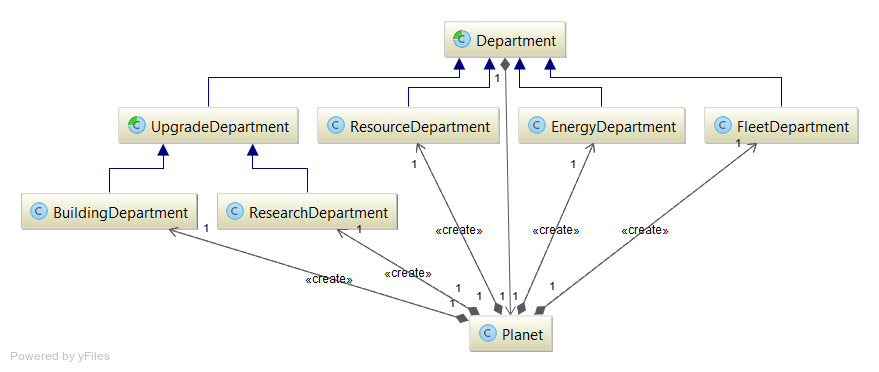
\includegraphics[scale=0.5]{diagram2.png}
\caption{Диаграмма классов  департаментов}
\label{pic:d1}
\end{figure}

Для представления зданий и исследований используются классы Building  и Research  соответственно. Эти классы реализуют интерфейс Upgradable , в котором объявлены методы позволяющие начать улучшение, узнать длительность улучшения, его стоимость и текущий уровень объекта.

Классы Building и Research содержат ссылку на соответствующий объект перечисления типа BuildingType   или
 ResearchType. Каждый объект перечисления содержит набор констант, на основе которых вычисляется время улучшения, его стоимость и длительность. Ссылка на объект перечисления передается в конструктор объекта, так в модели определяется тип постройки и исследования, а также часть его поведения.

По своей сути каждый объект одного из этих типа представляет собой хранилище для ссылка на соответствующий объект перечисления и уровня, в котором так же реализована логика расчета различных параметров. 

Корабли представлены классом Ship, реализующий интерфейс Constuctable. Отличие этого интерфейса от Upgradable состоит в том, что у объекта реализующего этот интерфейс нет уровня, а вместо улучшение происходит создание новых единиц.

В объекте класса Ship так же хранится ссылка на соответствующий объект перечисления типа ShipType, содержащий константы определяющие характеристики корабля такие как скорость, прочность, прочность щитов, скорость и вместимость. Класс Ship реализует логику расчета этих характеристик и постройки новых кораблей.

На характеристики кораблей, построек и исследований влияют не только их уровни, но и уровни других объектов, например, время улучшений исследований зависит от уровня здания лаборатории, а атака кораблей зависит от уровня исследования лазерной технологии. Чтобы реализовать такие зависимости, внутри объектов содержатся набор ссылок на объекты от которых зависят. Доступ к этим объектам обеспечивается с помощью департаментов. Каждый объект типа Ship, Building или Research имеет ссылку на соответствующий объект ShipDepartment, BuildingDepartment или ResearchDepartment. Так же логика улучшения или строительства основана на взаимодействии с департаментами.

Класс Fleet представляет флот. Флот реализован с помощью класса стандартной библиотеки Map в котором хранятся пары значений ShipType и Integer, каждая пара соответствует типу корабля и количеству кораблей данного типа во флоте. Флот поддерживает операции отделения и обледенения. Также флоты могут атаковать друг друга.

Ресурсы представлены классом Resource, в котором три поля целочисленного типа, соответствующее каждому из трех типов ресурсов. Ресурсы также поддерживают операции разделения и объединения.

Для реализации различных действий, таких как улучшение зданий и исследований, строительство кораблей, выполнение миссий и др. был использован паттерн проектирования "Команда". Таким образом, был создан абстрактный класс Action, который реализовывает данные паттерн. Внутри каждого объекта класса Action существует две очереди объектов этого же типа реализованные с помощью LinkedList. Так, существует возможность выполнять действия в определенной последовательности. 

Например, при инициировании обновления здания в модели создается объект типа Upgrade, который расширяет Action и содержит дополнительные сведения об улучшаемом объекте. Далее, этот объект передается в UpgradeDepartment, где создается анонимный класс расширяющий Action и добавляется в очередь команд объекта Upgrade. Добавляемая команда отвечает за изменение количества занятых полей на планете. Таким образом, при улучшении здании обязательно произойдут все необходимые действия. Подобные средства используются в других местах и на других уровнях. Это позволяет удобным и простым способом обеспечить правильную последовательность выполняемых действий в модели, а также облегчает расширение системы. 

\begin{figure}[H]
\centering
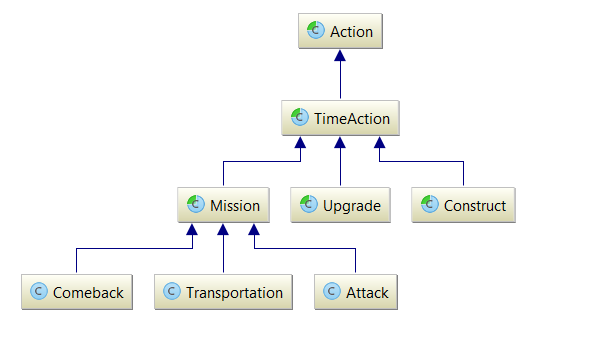
\includegraphics[scale=0.5]{d3.png}
\caption{Диаграмма классов  реализующий паттерн "Команда"}
\label{pic:d3}
\end{figure}

На рисунке \ref{pic:d3} представлена диаграмма классов, которые реализуюи описываемый паттерн.

\subsubsection{Графический интерфейс}
Для создания графического интерфейса применялась библиотека JavaFX.

\begin{figure}[H]
\centering
\begin{subfigure}[b]{0.4\textwidth} 
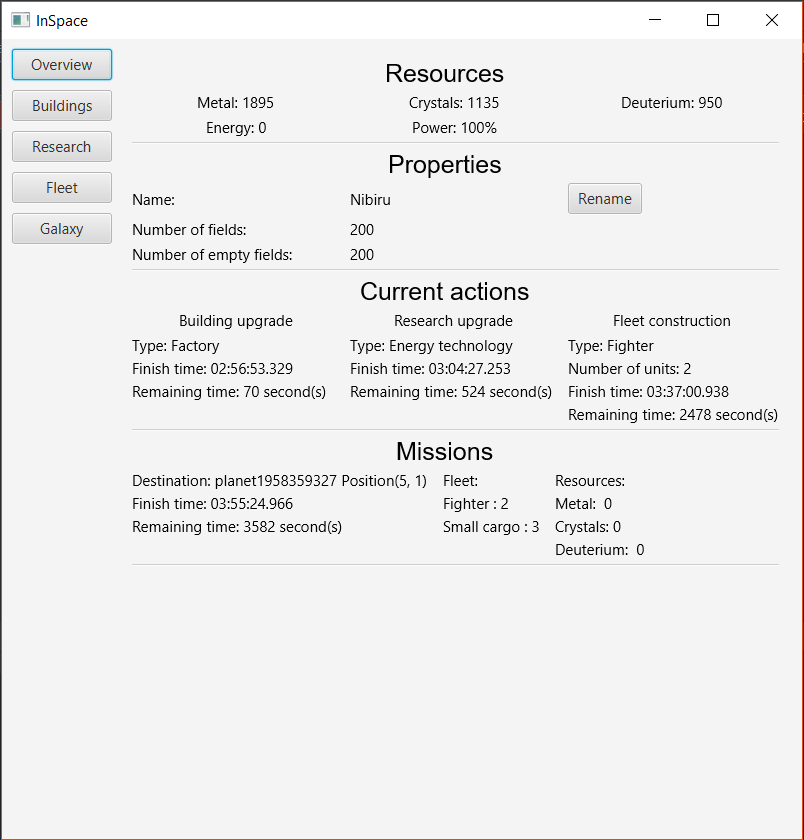
\includegraphics[width=1\textwidth]{../screenshots/1.png}
\caption{Обзор планеты}
\end{subfigure}
\begin{subfigure}[b]{0.4\textwidth} 
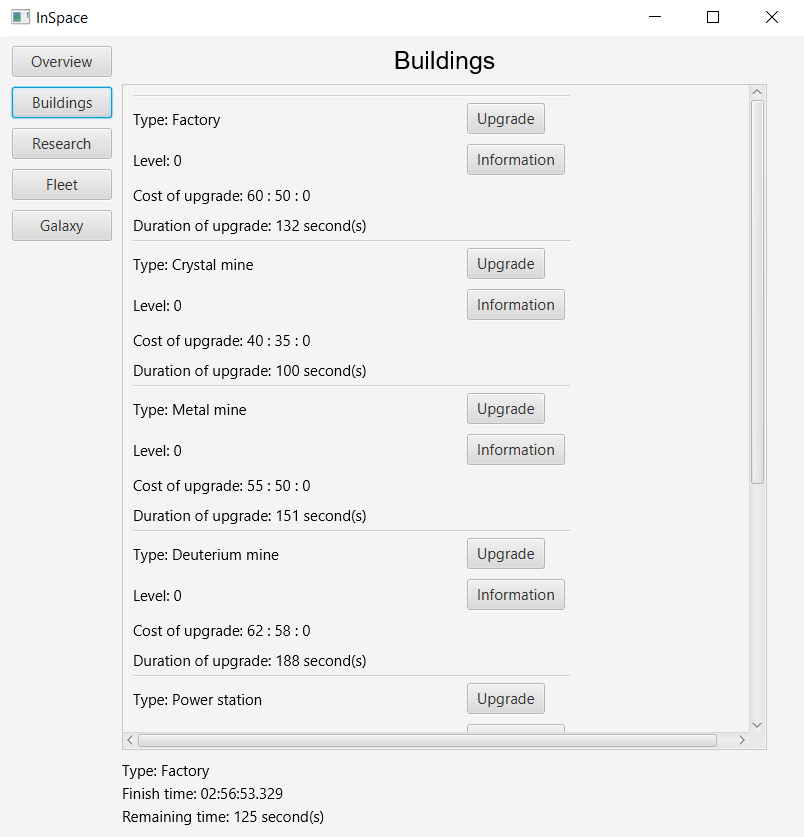
\includegraphics[width=1\textwidth]{../screenshots/2.png}
\caption{Список зданий}
\end{subfigure}
\begin{subfigure}[b]{0.4\textwidth} 
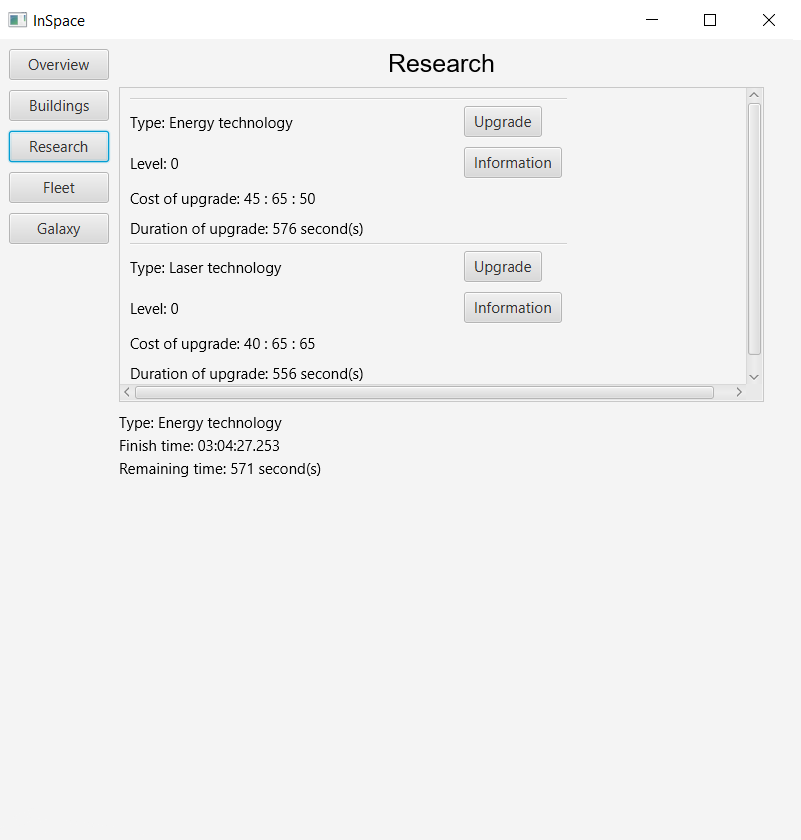
\includegraphics[width=1\textwidth]{../screenshots/3.png}
\caption{Список исследований}
\end{subfigure}
\begin{subfigure}[b]{0.4\textwidth} 
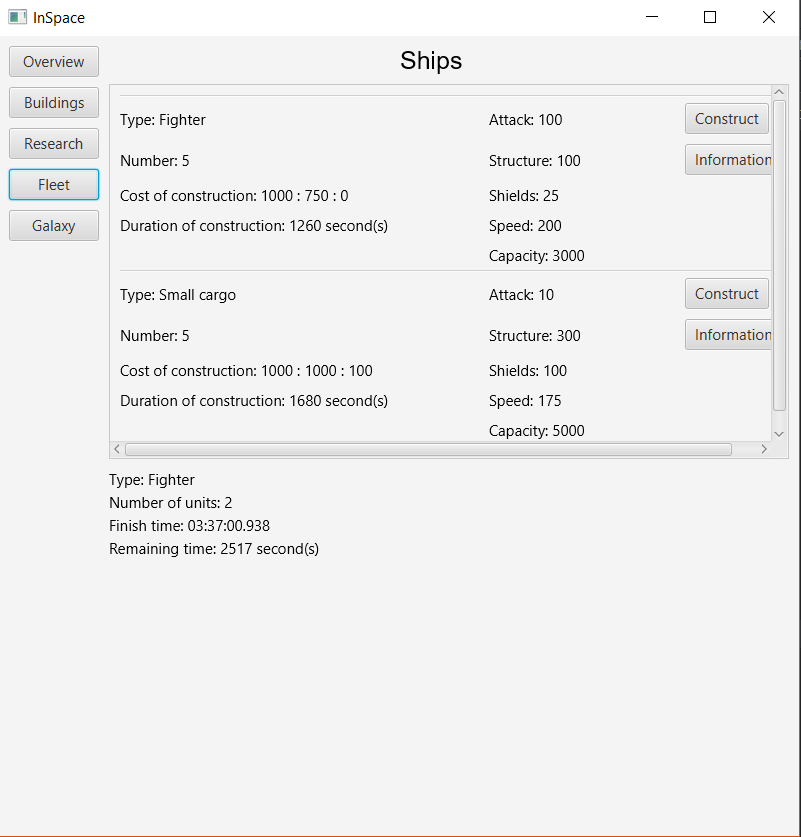
\includegraphics[width=1\textwidth]{../screenshots/4.png}
\caption{Список кораблей}
\end{subfigure}
\begin{subfigure}[b]{0.4\textwidth} 
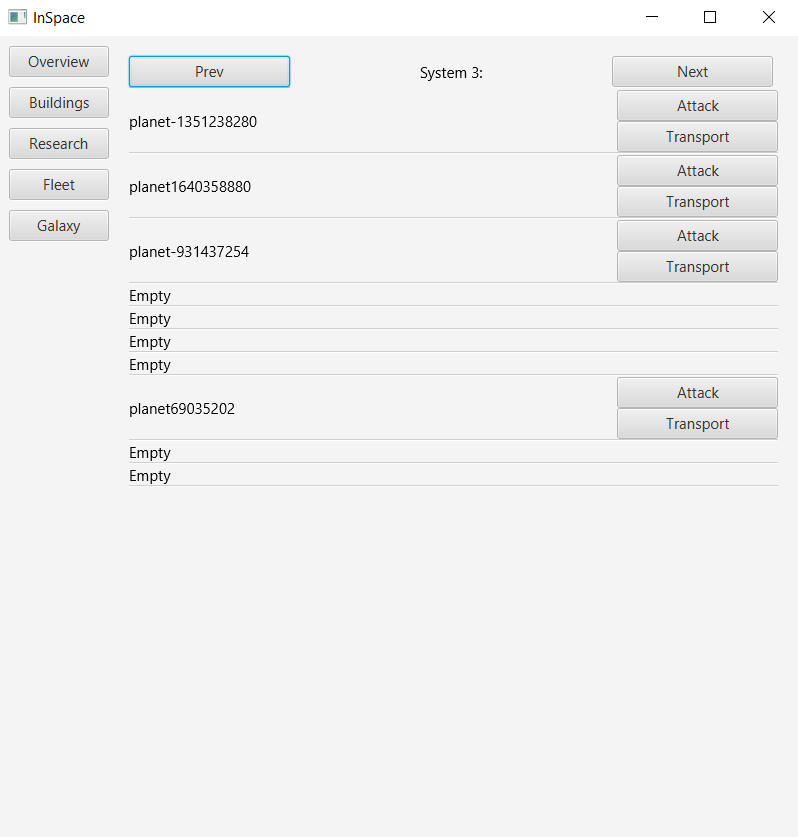
\includegraphics[width=1\textwidth]{../screenshots/5.png}
\caption{Обзор системы}
\end{subfigure}
\caption{Снимки экрана приложения}
\label{pic:gui}
\end{figure} 

Отображение элементов модели и взаимодействие с ними обеспечивалось объектами классов производных от Node. Для преобразования объектов библиотеки, представляющих какую-либо часть модели, в объекты типа Node были создан ряд классов-фабрик. Методы этих классов принимали в качестве аргументов ссылки на объекты модели и возвращали соответствующие объекты класса Node или производных от него. Полученные с помощью фабрик объекты компоновались и располагались на более высоком уровне. На рисунке \ref{pic:gui} изображены основные виды приложения.
%TODO


  

\subsection{Выводы}
Таким образом, основные компоненты приложения были реализованы. В ходе работы преследовалась цель создать понятную, легко расширяемую и дополняемую архитектуру. При реализации удалось применить паттерны объектно-ориентированного проектирования и использовать различные особенности языка такие, как анонимные классы, лямбда-выражения и др. 
%TODO
   
\section{Процесс обеспечения качества и тестирование приложения, реализующего космический симулятор InSpace}

В процессе разработки приложения для обеспечения качества были использованы различные инструменты и методики: автоматическое и ручное тестирование, статический анализ, просмотр кода и демонстрации.

\subsection{Автоматическое тестирование}

В ходе разработки проекта регулярно проводилось автоматическое тестирование. Для этого использовался фреймворк Junit 4.11, который упрощает написание тестирующего кода, а также предоставляет информацию о результатах тестирования в удобном виде, что позволяет ее систематизировать. Кроме того, для написания тестов использовалась мок-библиотека PowerMock 1.5.4. Подмена возвращаемых значений методов позволило протестировать большее количество возможных игровых ситуаций. 

В ходе разработки был написан функциональный тест, с помощью которого выполнялась проверка работоспособности основных функциональностей библиотеки. В итоге, покрытие тестами составило 86\%.

Тестирование позволило поддерживать работоспособность продукта в ходе всего процесса разработки, а также сильно упрощало поиск допущенных ошибок и обеспечивало их своевременное исправление.   

\subsection{Ручное тестирование}
Для проверки различных сценариев использования приложения также применялось ручное тестированные. Так с помощью графического интерфейса был смоделирован игровой цикл и проверены основные функциональности приложения такие как улучшение зданий и исследований, строительство кораблей, проведение миссий, накопление ресурсов и др. В ходе ручного тестирования в графическом интерфейсе был найден ряд ошибок, которые были впоследствии исправлены. 

\subsection{Статический анализ}

Для улучшения качества и надежности создаваемого продукта использовались средства для статического анализа кода.

Для статического анализа использовалась программа FindBugs 3.0.1. Данный инструмент производит анализ кода до момента компиляции и способен обнаруживать ряд ошибок связанных со стилем кода, производительностью конечного продукта и др. В ходе работы, полученные с помощью этого инструмента отчеты просматривались и найденные ошибки исправлялись, что позволило улучшить стиль написания кода.

\subsection{Непрерывная интеграция}

В ходе разработки активно использовались среды непрерывной интеграции Jenkins и Travis CI. Сборка проекта и запуск тестов в Jenkins осуществлялись c помощью плагина Pipeline посредством инструмента Docker. Для этого использовался контейнер \footnote{\url{https://hub.docker.com/r/lamtev/java/}}, который содержит все необходимые компоненты среды. Для Travis CI использовалось окружение Java и OracleJDK 8. При каждом обновления репозитория производилась полная сборка проекта, его тестирование и статический, а также собиралась различная статистическая информация. Использование непрерывной интеграции позволило контролировать состояние проекта на протяжении его создания.  
\subsection{Просмотр кода}

В ходе написания приложения производился просмотр кода, не участвующими в его создании людьми, которые высказывали свои замечания и предложения. Так, в ходе разработки было проведено 2 просмотра, нацеленных на выявление ошибок и недоработок, связанных  непосредственно с кодом, его стилем и архитектурой приложения. Первый просмотр был проведен 13.11.2016 одногруппником Ламтевым А.Ю., второй - 21.12.2016 преподавателем Вылегжаниной К.Д. В ходе данных проверок было получено большое количество различных замечаний, которые были в итоге исправлены. Так, довольно сильно были переработаны некоторые отвечающие за представление модели классы, взаимодействие между ними, а так же был изменен программный интерфейс библиотеки. Выполнение данных действий позволило сделать архитектуру приложения более простой и расширяемой, а также упростить работу с библиотекой.

\subsection{Демонстрации}

Во время создания приложения 1.12.2016 была проведена демонстрация, на которой были сделаны различные замечания и высказаны множество предложений и пожеланий, основанных на внешнем виде продукта и стандартном цикле работы с ним. Анализ полученной информации позволял обнаруживать недочеты присутствующие в продукте, а также определять дальнейшие направления для улучшения и расширения проекта. Список составленных на основе замечаний, полученных в ходе демонстрации, задач выглядит следующим образом:
\begin{itemize}
\item Исключить дублирование названия планет
\item Изменить отображение оставшегося времени с секунд на часы, минуты и секунды
\item Сделать отдельное отображение панели с ресурсами при любом содержании окна.
\item Заменить кнопки вкладками
\end{itemize}

Выполнение перечисленных задач, а также применение данной практики в будущем, безусловно, позволит улучшить приложение.

\subsection{Выводы}
Применяемые инструменты и методики позволили уменьшить ошибок и недоработок и облегчить дальнейшей расширение и улучшение приложения, путем обеспечения своевременного обнаружения новых ошибок. 

\section{Выводы}
В ходе работы были получены навыки необходимые для написания приложений на языке программирования Java. Была изучена стандартная библиотека и особенности данного языка.

Созданный продукт оказался работоспособным и удовлетворяет поставленным требованиям. Планируется продолжить работу по совершенствованию библиотеки и графического приложения, перейти к многопользовательской версии, использовать базу данных для хранения модели, создать веб-интерфейс.

\section{Приложение 1}
\label{sec:listings}

В данном приложение приведены листинги кода созданного приложения. Исходны ход можно найти в репеозитории\footnote{\url{https://github.com/lezhenin/InSpace}} на ресурсе GitHub.

\captionof{lstlisting}{Planet.java}
\label{listing:Galaxy} 
\lstinputlisting[label=code:hello]{../../core/src/main/java/ru/spbstu/icc/kspt/inspace/model/Galaxy.java}
\parindent=0.6cm


\captionof{lstlisting}{Planet.java}
\label{listing:Planet} 
\lstinputlisting[label=code:hello]{../../core/src/main/java/ru/spbstu/icc/kspt/inspace/model/Planet.java}
\parindent=0.6cm


\captionof{lstlisting}{Position.java}
\label{listing:Position} 
\lstinputlisting[label=code:hello]{../../core/src/main/java/ru/spbstu/icc/kspt/inspace/model/Position.java}
\parindent=0.6cm


\captionof{lstlisting}{Building.java}
\label{listing:Building} 
\lstinputlisting[label=code:hello]{../../core/src/main/java/ru/spbstu/icc/kspt/inspace/model/buildings/Building.java}
\parindent=0.6cm


\captionof{lstlisting}{BuildingType.java}
\label{listing:BuildingType} 
\lstinputlisting[label=code:hello]{../../core/src/main/java/ru/spbstu/icc/kspt/inspace/model/buildings/BuildingType.java}
\parindent=0.6cm


\captionof{lstlisting}{BuildingDepartment.java}
\label{listing:BuildingDepartment} 
\lstinputlisting[label=code:hello]{../../core/src/main/java/ru/spbstu/icc/kspt/inspace/model/buildings/BuildingDepartment.java}
\parindent=0.6cm


\captionof{lstlisting}{Research.java}
\label{listing:Research} 
\lstinputlisting[label=code:hello]{../../core/src/main/java/ru/spbstu/icc/kspt/inspace/model/research/Research.java}
\parindent=0.6cm


\captionof{lstlisting}{ResearchType.java}
\label{listing:ResearchType} 
\lstinputlisting[label=code:hello]{../../core/src/main/java/ru/spbstu/icc/kspt/inspace/model/research/ResearchType.java}
\parindent=0.6cm


\captionof{lstlisting}{ResearchDepartment.java}
\label{listing:ResearchDepartment} 
\lstinputlisting[label=code:hello]{../../core/src/main/java/ru/spbstu/icc/kspt/inspace/model/research/ResearchDepartment.java}
\parindent=0.6cm


\captionof{lstlisting}{Fleet.java}
\label{listing:Fleet} 
\lstinputlisting[label=code:hello]{../../core/src/main/java/ru/spbstu/icc/kspt/inspace/model/fleet/Fleet.java}
\parindent=0.6cm


\captionof{lstlisting}{Ship.java}
\label{listing:Ship} 
\lstinputlisting[label=code:hello]{../../core/src/main/java/ru/spbstu/icc/kspt/inspace/model/fleet/Ship.java}
\parindent=0.6cm


\captionof{lstlisting}{ShipType.java}
\label{listing:ShipType} 
\lstinputlisting[label=code:hello]{../../core/src/main/java/ru/spbstu/icc/kspt/inspace/model/fleet/ShipType.java}
\parindent=0.6cm


\captionof{lstlisting}{FleetDepartment.java}
\label{listing:FleetDepartment} 
\lstinputlisting[label=code:hello]{../../core/src/main/java/ru/spbstu/icc/kspt/inspace/model/fleet/FleetDepartment.java}
\parindent=0.6cm


\captionof{lstlisting}{Mission.java}
\label{listing:Mission} 
\lstinputlisting[label=code:hello]{../../core/src/main/java/ru/spbstu/icc/kspt/inspace/model/fleet/missions/Mission.java}
\parindent=0.6cm


\captionof{lstlisting}{Attack.java}
\label{listing:Attack} 
\lstinputlisting[label=code:hello]{../../core/src/main/java/ru/spbstu/icc/kspt/inspace/model/fleet/missions/Attack.java}
\parindent=0.6cm


\captionof{lstlisting}{Transportation.java}
\label{listing:Transortation} 
\lstinputlisting[label=code:hello]{../../core/src/main/java/ru/spbstu/icc/kspt/inspace/model/fleet/missions/Transportation.java}
\parindent=0.6cm


\captionof{lstlisting}{Comeback.java}
\label{listing:Comeback} 
\lstinputlisting[label=code:hello]{../../core/src/main/java/ru/spbstu/icc/kspt/inspace/model/fleet/missions/Comeback.java}
\parindent=0.6cm


\captionof{lstlisting}{Resources.java}
\label{listing:Resources} 
\lstinputlisting[label=code:hello]{../../core/src/main/java/ru/spbstu/icc/kspt/inspace/model/resources/Resources.java}
\parindent=0.6cm


\captionof{lstlisting}{ResourceProducer.java}
\label{listing:ResourceProducer} 
\lstinputlisting[label=code:hello]{../../core/src/main/java/ru/spbstu/icc/kspt/inspace/model/resources/ResourceProducer.java}
\parindent=0.6cm


\captionof{lstlisting}{ResourceDepartment.java}
\label{listing:ResourceDepartment} 
\lstinputlisting[label=code:hello]{../../core/src/main/java/ru/spbstu/icc/kspt/inspace/model/resources/ResourceDepartment.java}
\parindent=0.6cm


\captionof{lstlisting}{EnergyDepartment.java}
\label{listing:EnergyDepartment} 
\lstinputlisting[label=code:hello]{../../core/src/main/java/ru/spbstu/icc/kspt/inspace/model/energy/EnergyDepartment.java}
\parindent=0.6cm


\captionof{lstlisting}{EnergyProducer.java}
\label{listing:EnergyProducer} 
\lstinputlisting[label=code:hello]{../../core/src/main/java/ru/spbstu/icc/kspt/inspace/model/energy/EnergyProducer.java}
\parindent=0.6cm


\captionof{lstlisting}{EnergyConsumer.java}
\label{listing:EnergyConsumer} 
\lstinputlisting[label=code:hello]{../../core/src/main/java/ru/spbstu/icc/kspt/inspace/model/energy/EnergyConsumer.java}
\parindent=0.6cm


\captionof{lstlisting}{Department.java}
\label{listing:Department} 
\lstinputlisting[label=code:hello]{../../core/src/main/java/ru/spbstu/icc/kspt/inspace/model/utils/Department.java}
\parindent=0.6cm


\captionof{lstlisting}{UpgradeDepartment.java}
\label{listing:UpgradeDepartment} 
\lstinputlisting[label=code:hello]{../../core/src/main/java/ru/spbstu/icc/kspt/inspace/model/utils/UpgradeDepartment.java}
\parindent=0.6cm


\captionof{lstlisting}{Upgradable.java}
\label{listing:Upgradable} 
\lstinputlisting[label=code:hello]{../../core/src/main/java/ru/spbstu/icc/kspt/inspace/model/utils/Upgradable.java}
\parindent=0.6cm


\captionof{lstlisting}{Constructable.java}
\label{listing:Constructable} 
\lstinputlisting[label=code:hello]{../../core/src/main/java/ru/spbstu/icc/kspt/inspace/model/utils/Constructable.java}
\parindent=0.6cm


\captionof{lstlisting}{Action.java}
\label{listing:Action} 
\lstinputlisting[label=code:hello]{../../core/src/main/java/ru/spbstu/icc/kspt/inspace/model/utils/Action.java}
\parindent=0.6cm


\captionof{lstlisting}{TimeAction.java}
\label{listing:TimeAction} 
\lstinputlisting[label=code:hello]{../../core/src/main/java/ru/spbstu/icc/kspt/inspace/model/utils/TimeAction.java}
\parindent=0.6cm


\captionof{lstlisting}{Time.java}
\label{listing:Time} 
\lstinputlisting[label=code:hello]{../../core/src/main/java/ru/spbstu/icc/kspt/inspace/model/utils/Time.java}
\parindent=0.6cm


\captionof{lstlisting}{Upgrade.java}
\label{listing:Upgrade} 
\lstinputlisting[label=code:hello]{../../core/src/main/java/ru/spbstu/icc/kspt/inspace/model/utils/Upgrade.java}
\parindent=0.6cm


\captionof{lstlisting}{Construct.java}
\label{listing:Construct} 
\lstinputlisting[label=code:hello]{../../core/src/main/java/ru/spbstu/icc/kspt/inspace/model/utils/Construct.java}
\parindent=0.6cm


\captionof{lstlisting}{CapacityExcessException.java}
\label{listing:CapacityExcessException} 
\lstinputlisting[label=code:hello]{../../core/src/main/java/ru/spbstu/icc/kspt/inspace/model/exception/CapacityExcessException.java}
\parindent=0.6cm


\captionof{lstlisting}{CapacityExcessException.java}
\label{listing:CapacityExcessException} 
\lstinputlisting[label=code:hello]{../../core/src/main/java/ru/spbstu/icc/kspt/inspace/model/exception/CapacityExcessException.java}
\parindent=0.6cm

\captionof{lstlisting}{FleetDetachException.java}
\label{listing:FleetDetachException} 
\lstinputlisting[label=code:hello]{../../core/src/main/java/ru/spbstu/icc/kspt/inspace/model/exception/FleetDetachException.java}
\parindent=0.6cm


\captionof{lstlisting}{UpgradeException.java}
\label{listing:UpgradeException} 
\lstinputlisting[label=code:hello]{../../core/src/main/java/ru/spbstu/icc/kspt/inspace/model/exception/UpgradeException.java}
\parindent=0.6cm


\captionof{lstlisting}{build.gradle}
\label{listing:gradle} 
\lstinputlisting[label=code:hello]{../../build.gradle}
\parindent=0.6cm


\captionof{lstlisting}{app/build.gradle}
\label{listing:appgradle} 
\lstinputlisting[label=code:hello]{../../app/build.gradle}
\parindent=0.6cm

\captionof{lstlisting}{core/build.gradle}
\label{listing:coregradle} 
\lstinputlisting[label=code:hello]{../../core/build.gradle}
\parindent=0.6cm


\captionof{lstlisting}{Jenkinsfile}
\label{Jenkinsfile} 
\lstinputlisting[label=code:hello]{../../Jenkinsfile.}
\parindent=0.6cm


\captionof{lstlisting}{travis.yml}
\label{travis.yml} 
\lstinputlisting[label=code:hello]{../../.travis.yml}
\parindent=0.6cm

\end{document}